\documentclass[12pt]{article}

\usepackage{amsmath, amssymb, amsthm}
\usepackage{hyperref}
\usepackage{geometry}
\usepackage{booktabs}
\usepackage{graphicx}
\usepackage{draftwatermark}
\SetWatermarkText{WORKING PAPER}
\SetWatermarkScale{1.5}
\SetWatermarkAngle{45}
\SetWatermarkColor[gray]{0.80}
\geometry{margin=1in}

% Theorem environments
\newtheorem{theorem}{Theorem}[section]
\newtheorem{lemma}[theorem]{Lemma}
\newtheorem{proposition}[theorem]{Proposition}
\newtheorem{corollary}[theorem]{Corollary}
\theoremstyle{definition}
\newtheorem{definition}[theorem]{Definition}
\theoremstyle{remark}
\newtheorem{remark}[theorem]{Remark}

% Notation
\newcommand{\vt}{v_2}
\newcommand{\Sm}{S}

\title{First-Principles Derivation of the Steiner Sentence Length Distribution\\[0.5em]
       \large Speculative Results Series, Paper~67}

\author{Jon Seymour\\
  \texttt{jon@wildducktheories.com}\\
  Sydney, Australia}
\date{July 2026}

\begin{document}

\maketitle

\begin{abstract}
We prove that Steiner sentences in the Syracuse graph have length
distribution $P(\text{sentence length} = k) = 3^{k-1}/4^k$ for all $k \geq 1$.
The proof proceeds in three steps.
First, we establish the exact Syracuse transition matrix on residue
classes modulo~8 from arithmetic alone: the mod-8 map is uniform from
classes~1 and~5, while classes~3 and~7 have restricted (forbidden) transitions
determined by mod-16 arithmetic.
Second, we identify the invariant $d_3 = d_7$ — equal weight on classes~3
and~7 in the surviving (non-terminated) distribution — and show it is
preserved by the transition matrix unconditionally, for any value of $d_1$.
Third, we show that the invariant $d_3 = d_7$ is precisely the algebraic
condition under which the surviving mass decays by exactly~$3/4$ per step,
giving $P(k) = 3^{k-1}/4^k$.

The proof requires no ergodic theory and no appeal to the Collatz conjecture.
It is a direct consequence of two classical arithmetic facts: that
$3n+1 \equiv 2 \pmod{4}$ for $n \equiv 3$ or $7 \pmod 8$ (mod-8 forbidden
transitions), and that multiplication by~3 is a bijection on
$\mathbb{Z}/2^j\mathbb{Z}$ (uniform distribution from classes~1 and~5).

Appendix~A provides a complete empirical validation: $10^5$ sentences sampled
uniformly over $[1, 10^{15}]$, the sentence-start distribution, the within-sentence
word entry distribution, the sentence length table comparing the naive $(1/2)^k$
prediction and the theoretical $3^{k-1}/4^k$, and $\chi^2$ goodness-of-fit tests.
The naive prediction is rejected with $\chi^2 \approx 10^6$; the theoretical formula
is consistent ($p \approx 0.61$).

\medskip
\noindent\textbf{Status.} This paper contains proved theorems and complete empirical
validation. All theoretical results are unconditional.
\end{abstract}

\tableofcontents

% ---------------------------------------------------------------------------
\section{Background and Notation}
\label{sec:background}

We work throughout with odd positive integers.

\begin{definition}[Syracuse map]
\label{def:syracuse}
The \emph{Syracuse map} $\Sm : \mathbb{O} \to \mathbb{O}$ on odd positive
integers is
\[
  \Sm(n) \;=\; \frac{3n+1}{2^{\vt(3n+1)}},
\]
where $\vt(m)$ denotes the 2-adic valuation of $m$.
\end{definition}

\begin{definition}[Steiner sentence]
\label{def:sentence}
A \emph{Steiner sentence} is a maximal sequence of consecutive applications of~$\Sm$
from an initial node $b_0 = \Sm(n)$ with $n \equiv 5 \pmod{8}$, terminating at
the first node $b_k \equiv 5 \pmod{8}$. The \emph{sentence length} is the number
of steps~$k$.
\end{definition}

\begin{remark}
Steiner sentences are the fundamental composite building blocks of Collatz paths; see
Paper~33~\cite{paper33} for the full Steiner circuit framework.
The sentence start $b_0 = \Sm(n)$ is the node immediately following a $5 \pmod 8$
node in the orbit, and the sentence ends at the next $5 \pmod 8$ node.
\end{remark}

\begin{remark}[Why Steiner sentences are the right scale]
\label{rem:scale}
The Steiner sentence decomposition is chosen precisely so that class~$5 \pmod 8$
is \emph{always a sink and never a source} within a sentence.
This has a crucial arithmetic consequence.

For $n \equiv 1, 3, 7 \pmod 8$, the 2-adic valuation $\vt(3n+1)$ is a
\emph{constant} determined entirely by $n \bmod 8$: it equals~2, 1, and~1
respectively (Paper~66~\cite{paper66}, Theorem~2.1).
The Syracuse image $\Sm(n) \bmod 8$ is therefore completely determined by
$n \bmod 8$ alone, with exact rational transition probabilities.

For $n \equiv 5 \pmod 8$, by contrast, $\vt(3n+1) = 3 + \vt(3k+2)$ where
$n = 8k+5$, and $\vt(3k+2)$ is an unbounded random variable whose
expectation requires summing a geometric series (Paper~66).
The transition probabilities out of class~5 are still exactly $1/4$ each,
but they arise from a distribution over infinitely many valuation values,
not a single fixed shift.

By restricting to the \emph{interior} of a sentence —
the steps from $b_0 \not\equiv 5$ to the terminal word —
class~5 never appears as a source.
The surviving chain operates entirely on $\{1,3,7\}$, where every
valuation is a constant and every transition probability is an exact rational.
The variable-valuation complexity of class~5 is absorbed at the sentence
boundary and plays no role in the counting argument.
This is why the sentence length distribution $3^{k-1}/4^k$ admits a
clean closed-form proof: at the scale of Steiner sentences, the arithmetic
is exact.
\end{remark}

Paper~65~\cite{paper65} was the first attempt at this subject.
It observed empirically that
$P(\text{sentence length} = k) = \frac{1}{3}(3/4)^k$,
equivalently $3^{k-1}/4^k$, and stated the result as a conjecture.
The present paper supersedes Paper~65 by providing a complete proof,
and incorporates its experimental record in Appendix~A.

% ---------------------------------------------------------------------------
\section{The Syracuse Transition Matrix mod~8}
\label{sec:matrix}

We model the sentence as a Markov chain on residue classes modulo~8.
The transition probability $P[a][b]$ is the natural density of odd integers
$n \equiv a \pmod{8}$ for which $\Sm(n) \equiv b \pmod{8}$,
i.e.\ $P[a][b] = \lim_{N\to\infty} \frac{1}{N}\#\{n \leq N : n \equiv a, \Sm(n) \equiv b \pmod 8\}$.
All results in this paper are unconditional: they require no assumption beyond this
standard density definition and do not depend on the Collatz conjecture.

\begin{theorem}[Syracuse transition matrix mod~8]
\label{thm:matrix}
The transition matrix on $\{1, 3, 5, 7\} \pmod{8}$ is:
\[
P \;=\;
\begin{array}{c|cccc}
   & 1   & 3   & 5   & 7   \\
\hline
1  & 1/4 & 1/4 & 1/4 & 1/4 \\
3  & 1/2 & 0   & 1/2 & 0   \\
5  & 1/4 & 1/4 & 1/4 & 1/4 \\
7  & 0   & 1/2 & 0   & 1/2 \\
\end{array}
\]
(rows = source class, columns = target class).
\end{theorem}

\begin{proof}
We prove each row by direct arithmetic.

\medskip\noindent
\textbf{Row 1 (uniform).}
Write $n = 8k+1$. Then $3n+1 = 24k+4 = 4(6k+1)$.
Since $6k+1$ is always odd, $\vt(3n+1) = 2$ exactly and $\Sm(n) = 6k+1$.
Now $6k+1 \pmod 8$: as $k$ runs through $0,1,2,3 \pmod 4$, we get
$6k+1 \equiv 1,7,5,3 \pmod 8$ respectively.
Each residue in $\{1,3,5,7\}$ appears with equal density, so $P[1][b] = 1/4$
for all $b \in \{1,3,5,7\}$.

\medskip\noindent
\textbf{Row 5 (uniform).}
Write $n = 8k+5$. Then $3n+1 = 8(3k+2)$, so $\vt(3n+1) = 3 + \vt(3k+2)$.
Write $3k+2 = 2^m q$ with $q$ odd; then $\Sm(n) = q$.
We need $q \pmod 8$ to be uniform on $\{1,3,5,7\}$.

Since $\gcd(3, 2^j) = 1$ for all $j \geq 1$, the map $k \mapsto 3k+2$ is
a bijection on $\mathbb{Z}/2^j\mathbb{Z}$.
As $k$ ranges over any $2^{j+3}$ consecutive integers, the value $3k+2$
hits each residue class mod $2^{j+3}$ exactly $2^j$ times.
In particular, as $k$ ranges over $\{0, 1, \ldots, 2^N - 1\}$, the value
$\Sm(8k+5) \pmod 8$ is uniform over $\{1,3,5,7\}$: for each target residue
$b \in \{1,3,5,7\}$ there are exactly $2^{N-2}$ values of $k$ giving
$\Sm(n) \equiv b \pmod 8$, as proved in Theorem~2.1(3) and Proposition~4.1
of Paper~66~\cite{paper66} via the same bijectivity argument.
Thus $P[5][b] = 1/4$ for all $b \in \{1,3,5,7\}$.

\medskip\noindent
\textbf{Row 3 (restricted to $\{1, 5\}$).}
Write $n = 8k+3$. Then $3n+1 = 24k+10 = 2(12k+5)$.
Since $12k$ is even, $12k+5$ is always odd, so $\vt(3n+1) = 1$ exactly
and $\Sm(n) = 12k+5$.
Now $12k+5 \pmod 8$: $12k \equiv 4k \pmod 8$, so $12k+5 \equiv 4k+5 \pmod 8$.
For $k$ odd: $4k \equiv 4 \pmod 8$, giving $12k+5 \equiv 1 \pmod 8$.
For $k$ even: $4k \equiv 0 \pmod 8$, giving $12k+5 \equiv 5 \pmod 8$.
Since $k$ is odd and even with equal density, $P[3][1] = P[3][5] = 1/2$
and $P[3][3] = P[3][7] = 0$.

\medskip\noindent
\textbf{Row 7 (restricted to $\{3, 7\}$).}
Write $n = 8k+7$. Then $3n+1 = 24k+22 = 2(12k+11)$.
Since $12k+11$ is always odd, $\vt(3n+1) = 1$ exactly and $\Sm(n) = 12k+11$.
Now $12k+11 \pmod 8$: $12k+11 \equiv 4k+3 \pmod 8$.
For $k$ odd: $4k \equiv 4$, giving $4k+3 \equiv 7 \pmod 8$.
For $k$ even: $4k \equiv 0$, giving $4k+3 \equiv 3 \pmod 8$.
Therefore $P[7][3] = P[7][7] = 1/2$ and $P[7][1] = P[7][5] = 0$.
\end{proof}

\begin{remark}[Forbidden transitions]
The zero entries in $P$ — transitions $3 \to 3$, $3 \to 7$, $7 \to 1$,
$7 \to 5$ — are \emph{structurally forbidden} for all $n$, not just on
average. Classes~3 and~7 each map into a strict subset of $\{1,3,5,7\}$.
This structural restriction is the engine of the proof.
\end{remark}

\begin{remark}[The surviving chain has exact arithmetic]
\label{rem:exact}
Row~5 of~$P$ is never used in the proof of Theorem~\ref{thm:main}.
Within a sentence, class~5 is a sink: once the chain reaches~5
the sentence ends, and class~5 never acts as a source for subsequent steps.
The surviving distribution (Definition~\ref{def:surviving}) propagates
mass only through rows~1, 3, and~7 of~$P$.

For these three rows, all transition probabilities are \emph{exact rational
constants} that follow directly from $n \bmod 8$ alone:
$\vt(3n+1) = 2$ always for class~1, and $\vt(3n+1) = 1$ always for
classes~3 and~7.
No geometric series, no expectation, no appeal to the distribution of
$\vt(3n+1)$ for class~5 is ever needed.
The variable-valuation behaviour of class~5 — which requires an
infinite geometric series to characterise (Paper~66~\cite{paper66}) —
is invisible to the surviving chain.
This exactness is what makes the sentence decomposition the right scale
for counting, and what makes the proof of Theorem~\ref{thm:main} purely
algebraic.
\end{remark}

% ---------------------------------------------------------------------------
\section{The Sentence as a First-Passage Problem}
\label{sec:firstpassage}

A sentence is the first-passage time of the Markov chain $(P, \pi_0)$ to
state~$5$, where $\pi_0$ is the sentence-start distribution.

\begin{lemma}[Sentence-start distribution]
\label{lem:start}
The sentence-start distribution is
$\pi_0 = (1/4, 1/4, 1/4, 1/4)$ — uniform on $\{1,3,5,7\}$.
\end{lemma}

\begin{proof}
The sentence starts at $b_0 = \Sm(n)$ with $n \equiv 5 \pmod 8$.
By Theorem~\ref{thm:matrix}, row~5 of~$P$ is uniform,
so $b_0 \bmod 8$ is uniform on $\{1,3,5,7\}$.
\end{proof}

The sentence terminates at the first step where the chain visits state~$5$.
The sentence length $k$ is this first-passage time.

\begin{definition}[Surviving distribution]
\label{def:surviving}
Let $d_s^{(k)}$ denote the probability that the chain is at state~$s$
after $k$ steps without having visited state~5. Formally,
$d_s^{(0)} = \pi_0(s)$ and for $k \geq 0$:
\[
  d_s^{(k+1)} \;=\; \sum_{t \neq 5} d_t^{(k)} P[t][s],
  \qquad s \neq 5.
\]
The \emph{surviving mass} is $M_k = \sum_{s \neq 5} d_s^{(k)}$.
\end{definition}

The sentence length distribution follows from the surviving mass:
$M_{k-1}$ is the probability of surviving past step $k-1$, and $M_k$
is the probability of surviving past step $k$, so
\[
  P(\text{sentence length} = k) \;=\; M_{k-1} - M_k.
\]
Expanding: $M_{k-1} - M_k = \sum_{s \neq 5} d_s^{(k-1)} - \sum_{s \neq 5} d_s^{(k)}
= \sum_{t \neq 5} d_t^{(k-1)}\!\left(1 - \sum_{s \neq 5} P[t][s]\right)
= \sum_{t \neq 5} d_t^{(k-1)} P[t][5]$.

% ---------------------------------------------------------------------------
\section{The Invariant $d_3 = d_7$}
\label{sec:invariant}

The key structural fact is a symmetry between classes~3 and~7 in the
surviving distribution.

\begin{lemma}[Invariant]
\label{lem:invariant}
$d_3^{(k)} = d_7^{(k)}$ for all $k \geq 0$.
\end{lemma}

\begin{proof}
By Definition~\ref{def:surviving}, the surviving distribution sums only
over sources $t \neq 5$; class~5 contributes nothing because once the
chain reaches~5 the sentence terminates (the mass is absorbed, not
propagated). The transition update for states~3 and~7 is therefore:
\begin{align*}
d_3^{(k+1)} &= d_1^{(k)} \cdot P[1][3] + d_3^{(k)} \cdot P[3][3] + d_7^{(k)} \cdot P[7][3] \\
             &= \tfrac{1}{4}\,d_1^{(k)} + 0 \cdot d_3^{(k)} + \tfrac{1}{2}\,d_7^{(k)}, \\[4pt]
d_7^{(k+1)} &= d_1^{(k)} \cdot P[1][7] + d_3^{(k)} \cdot P[3][7] + d_7^{(k)} \cdot P[7][7] \\
             &= \tfrac{1}{4}\,d_1^{(k)} + 0 \cdot d_3^{(k)} + \tfrac{1}{2}\,d_7^{(k)}.
\end{align*}
The two expressions are identical: $d_3^{(k+1)} = d_7^{(k+1)}$ for any
$d_1^{(k)}, d_3^{(k)}, d_7^{(k)}$.
By induction, since $d_3^{(0)} = d_7^{(0)} = 1/4$ (Lemma~\ref{lem:start}),
$d_3^{(k)} = d_7^{(k)}$ for all $k \geq 0$.
\end{proof}

\begin{remark}[Structural source of the invariant]
The invariant holds because columns~3 and~7 of~$P$, restricted to rows
$\{1,3,7\}$, are \emph{identical}:
\[
  P[\cdot][3]\big|_{\{1,3,7\}} \;=\; P[\cdot][7]\big|_{\{1,3,7\}}
  \;=\; \bigl(\tfrac{1}{4},\, 0,\, \tfrac{1}{2}\bigr).
\]
This column symmetry is a direct consequence of Theorem~\ref{thm:matrix}:
\begin{itemize}
  \item \emph{From class~1}: uniform output gives equal weight $1/4$ to both~3 and~7.
  \item \emph{From class~3}: forbidden to reach~3 or~7 (both have weight~0).
  \item \emph{From class~7}: reaches~3 and~7 with equal probability~$1/2$ each.
\end{itemize}
The invariant is unconditional — it holds for \emph{any} value of $d_1$,
not just at the fixed point of the chain.
\end{remark}

% ---------------------------------------------------------------------------
\section{Main Theorem}
\label{sec:main}

\begin{theorem}[Sentence length distribution]
\label{thm:main}
For any $k \geq 1$:
\[
  P(\text{sentence length} = k) \;=\; \frac{3^{k-1}}{4^k}.
\]
Equivalently, $P(\text{sentence length} = k) = \frac{1}{3}\left(\frac{3}{4}\right)^k$.
\end{theorem}

\begin{proof}
We use the splitting: $P(\text{sentence length} = 1) = \pi_0(5) = 1/4$ (sentences
that start at $b_0 \equiv 5$ terminate immediately). For $k \geq 2$,
the sentence does not terminate at step~1 (probability $3/4$) and then
terminates at step $k-1$ from the conditional start, i.e.\
$P(\text{length} = k) = \tfrac{3}{4} \cdot g_{k-1}$,
where $g_j$ is the first-passage probability to~5 starting from the
conditional distribution $\pi_0(\,\cdot \mid \cdot \neq 5) = (1/3, 1/3, 1/3)$
uniform on $\{1,3,7\}$.

It suffices to show $g_j = (3/4)^{j-1}/4$ for all $j \geq 1$,
which follows if the surviving mass $M_j$ starting from uniform
$\{1,3,7\}$ satisfies $M_j = (3/4)^j$.

\medskip
\noindent\textbf{Step 1: $d_3 = d_7$ is preserved.}
The conditional start has $d_3^{(0)} = d_7^{(0)} = 1/3$, so
Lemma~\ref{lem:invariant} applies: $d_3^{(k)} = d_7^{(k)}$ for all $k \geq 0$.

\medskip
\noindent\textbf{Step 2: Surviving mass decays by exactly $3/4$.}
From Definition~\ref{def:surviving}, $M_{k+1} = \sum_{s \neq 5} d_s^{(k+1)}
= \sum_{s \neq 5}\sum_{t \neq 5} d_t^{(k)} P[t][s]
= \sum_{t \neq 5} d_t^{(k)} \sum_{s \neq 5} P[t][s]
= \sum_{t \neq 5} d_t^{(k)}(1 - P[t][5])$, giving:
\[
  M_{k+1} \;=\; d_1^{(k)}\bigl(1 - P[1][5]\bigr)
               + d_3^{(k)}\bigl(1 - P[3][5]\bigr)
               + d_7^{(k)}\bigl(1 - P[7][5]\bigr).
\]
Substituting $P[1][5] = 1/4$, $P[3][5] = 1/2$, $P[7][5] = 0$:
\[
  M_{k+1} \;=\; \tfrac{3}{4}\,d_1^{(k)} + \tfrac{1}{2}\,d_3^{(k)} + d_7^{(k)}.
\]
We claim $M_{k+1} = \tfrac{3}{4} M_k = \tfrac{3}{4}(d_1^{(k)} + d_3^{(k)} + d_7^{(k)})$.
This requires:
\[
  \tfrac{3}{4}\,d_1^{(k)} + \tfrac{1}{2}\,d_3^{(k)} + d_7^{(k)}
  \;=\; \tfrac{3}{4}\,d_1^{(k)} + \tfrac{3}{4}\,d_3^{(k)} + \tfrac{3}{4}\,d_7^{(k)},
\]
which simplifies to $\tfrac{1}{2}d_3^{(k)} + d_7^{(k)} = \tfrac{3}{4}(d_3^{(k)} + d_7^{(k)})$,
i.e.\ $d_7^{(k)} = d_3^{(k)}$. This is exactly Lemma~\ref{lem:invariant}.

\medskip
\noindent\textbf{Step 3: Initial condition.}
At $k = 0$, $M_0 = 1$ (the full conditional mass on $\{1,3,7\}$).
By induction, $M_k = (3/4)^k$ for all $k \geq 0$.

\medskip
\noindent\textbf{Conclusion.}
$g_j = M_{j-1} - M_j = (3/4)^{j-1} - (3/4)^j = (3/4)^{j-1}(1/4) = 3^{j-1}/4^j$.
Therefore:
\[
  P(\text{length} = 1) \;=\; \tfrac{1}{4} \;=\; \tfrac{3^0}{4^1},
\]
\[
  P(\text{length} = k) \;=\; \tfrac{3}{4} \cdot g_{k-1}
  \;=\; \tfrac{3}{4} \cdot \frac{3^{k-2}}{4^{k-1}}
  \;=\; \frac{3^{k-1}}{4^k}, \qquad k \geq 2.
\]
Both cases give $3^{k-1}/4^k$, completing the proof.
\end{proof}

\begin{corollary}[Normalisation]
$\sum_{k=1}^{\infty} P(\text{sentence length} = k) = 1$.
\end{corollary}

\begin{proof}
$\sum_{k=1}^{\infty} \frac{3^{k-1}}{4^k} = \frac{1}{4} \sum_{k=1}^{\infty} \left(\frac{3}{4}\right)^{k-1}
= \frac{1}{4} \cdot \frac{1}{1 - 3/4} = 1$.
\end{proof}

% ---------------------------------------------------------------------------
\section{Discussion}
\label{sec:discussion}

\subsection{The role of class~5}

The formula $3^{k-1}/4^k$ is the geometric distribution with success
probability~$1/4$, as if at each step the chain draws uniformly from
$\{1,3,5,7\}$ and terminates on drawing~5.
This appearance is striking because class~5 plays three distinct and
mutually reinforcing roles in the sentence structure.

\textbf{Class~5 as the termination state.}
A sentence terminates exactly when it reaches a node $\equiv 5 \pmod 8$.
Since class~5 is the unique absorbing boundary of the chain (once the
chain visits class~5, the sentence ends), it is structurally absent
from all intermediate steps.
Empirically, class~5 accounts for only $\approx 6.2\%$ of within-sentence
word entries (Appendix~A, Table~\ref{tab:entry}) — one entry per sentence,
uniformly distributed across sentence lengths — rather than the
$25\%$ it would contribute if words were unrestricted.

\textbf{Class~5 as the uniform source.}
The sentence starts at $b_0 = \Sm(n)$ with $n \equiv 5 \pmod 8$.
By row~5 of the transition matrix (Theorem~\ref{thm:matrix}), class~5
maps uniformly over $\{1,3,5,7\}$: any of the four classes is equally
likely as the first word.
In particular, exactly $1/4$ of sentences have $b_0 \equiv 5$, meaning
length~$k=1$. This is the correct $P(k=1) = 1/4$, not the naive $1/2$.
Class~5 is the unique class for which $\vt(3n+1) \geq 3$ always
(proved in Paper~66~\cite{paper66}), which forces the extra halvings
that spread the output uniformly.

\textbf{Class~5 as the structural asymmetry.}
The transition $7 \to 5$ is structurally forbidden: $P[7][5] = 0$.
Class~5 is therefore unreachable in one step from class~7,
while it is reachable from classes~1 (with probability~$1/4$) and~3
(with probability~$1/2$).
This asymmetry — class~5 reachable from some classes but not others — is
precisely what forces the invariant $d_3 = d_7$: nodes in class~7 can
only reach class~5 via a detour through class~3 or class~7, never directly.
The proof in Section~\ref{sec:invariant} shows that this forced detour
maintains equal weight on classes~3 and~7 throughout the chain, and
Section~\ref{sec:main} shows that this equal weight is the algebraic
condition that makes the effective termination probability exactly $1/4$
at every step, regardless of the current value of $d_1$.

\subsection{Connection to Paper~66}

Paper~66~\cite{paper66} proves that $E[\vt(3n+1) \mid n \equiv r \pmod 8]$
equals exactly 2, 1, 4, 1 for $r = 1,3,5,7$ respectively.
The two papers are complementary: Paper~66 establishes what happens \emph{at}
the class~5 boundary (a geometrically distributed valuation requiring an
infinite series for its expectation), while the present paper shows that by
choosing Steiner sentences as the unit of analysis, the class~5 boundary
need never be crossed from the inside — it only needs to be \emph{entered}.

More precisely, the $3/4$ decay rate follows from three facts, each drawing
on the same underlying arithmetic:
\begin{itemize}
  \item The $1/4$ probability of immediate termination ($b_0 \equiv 5$)
        uses row~5 of~$P$ exactly once — at the sentence start.
        Class~5 is the unique class with $c_r \geq 3$ (Paper~66), forcing
        the extra halvings that make its output uniform.
        This is the only point where the geometric-series character of
        class~5 is relevant.
  \item The $1/2$ termination probability from class~3 comes from the mod-16
        split of Theorem~\ref{thm:matrix}: $\vt(3n+1) = 1$ exactly for all
        $n \equiv 3 \pmod 8$, so $\Sm(n) \bmod 8$ is determined by $n \bmod 16$
        alone, with no random valuation.
  \item The invariant $d_3 = d_7$ — and hence the $3/4$ decay — involves
        classes~1, 3, and~7 only, all of which have constant valuations.
        The proof is purely algebraic: no expectation, no series.
\end{itemize}
Paper~66 handles the hard case (class~5, variable valuation).
Paper~67 sidesteps it by construction.

\subsection{Why $3^{k-1}/4^k$ rather than $(1/2)^k$}

The naive prediction $(1/2)^k$ arises from the ``3-node coin flip'' model:
treat each word in the sentence as independently terminating whenever
it visits the 3-node, with the 3-node split giving probability~$1/2$.
Under this model only classes~3 and~7 can terminate, and if the
within-sentence distribution were uniform over $\{1,3,5,7\}$, the
effective per-step termination probability would be:
\[
  \tfrac{1}{4}\cdot 0 \;+\; \tfrac{1}{4}\cdot\tfrac{1}{2}
  \;+\; \tfrac{1}{4}\cdot 1 \;+\; \tfrac{1}{4}\cdot\tfrac{1}{2}
  \;=\; \tfrac{1}{2},
\]
where the terms correspond to classes~1 (never terminates via 3-node),
3 (terminates with prob~$1/2$), 5 (terminal by definition), and 7
(terminates with prob~$1/2$).
This model is wrong in two ways.
First, class~1 \emph{can} reach class~5 directly: $P[1][5] = 1/4$,
so the naive assignment of~0 to class~1 understates termination from class~1.
Second and more importantly, class~7 \emph{cannot} reach class~5 at all:
$P[7][5] = 0$, so the naive assignment of~$1/2$ to class~7 overstates it.
The net effect of these two corrections is a reduction in the effective
termination rate from~$1/2$ to~$1/4$.
The structural reason is the forbidden transition $7 \to 5$:
a chain in class~7 must first transit to class~3 or~7 (remaining in
the growth classes), where it may then reach class~5 on a subsequent step.
The invariant $d_3 = d_7$ (Lemma~\ref{lem:invariant}) shows that
these two errors cancel exactly and yield an effective rate of precisely
$1/4$, independent of $d_1$.

% ---------------------------------------------------------------------------
\section*{Acknowledgements}

This paper is part of the speculative results stream (64+k) of the Collatz
programme. The proof structure was found through numerical exploration in
\texttt{notebooks/steiner-branch-model.ipynb}.

% ---------------------------------------------------------------------------
\appendix

\section{Empirical Validation}
\label{app:empirical}

This appendix records the complete numerical experiment establishing the sentence
length distribution. The experiment was first reported in Paper~65~\cite{paper65}
and is reproduced here in full as the empirical record accompanying this paper's proof.

\subsection*{Sampling Protocol}

\begin{enumerate}
  \item Draw $t$ uniformly at random from $[1, T_{\max}]$ with $T_{\max} = 10^{15}$.
  \item Set $n = 8t + 5$ (so $n \equiv 5 \pmod{8}$).
  \item Compute $b_0 = \Sm(n)$, the first Steiner word of the new sentence.
  \item Follow consecutive Steiner circuits from $b_0$, counting words, until
        the first output $b \equiv 5 \pmod{8}$. Record the word count as $k$.
\end{enumerate}

$N = 10^5$ independent sentences were collected with seed~42. Independence between
samples is ensured by the random draw of~$t$; no orbit tails are shared.

\subsection*{Sentence-start Distribution}

By Theorem~\ref{thm:matrix}, row~5 of~$P$ is uniform, so $b_0 = \Sm(n) \bmod 8$
should be uniform on $\{1,3,5,7\}$.

\begin{table}[h]
\centering
\begin{tabular}{rrrr}
\toprule
$b_0 \bmod 8$ & Count & Observed fraction & Expected (uniform) \\
\midrule
1 & 25181 & 0.25181 & 0.25000 \\
3 & 25023 & 0.25023 & 0.25000 \\
5 & 24852 & 0.24852 & 0.25000 \\
7 & 24944 & 0.24944 & 0.25000 \\
\bottomrule
\end{tabular}
\caption{Sentence-start distribution: $b_0 = \Sm(n)$, $n \equiv 5\pmod{8}$,
$N = 10^5$ samples. The distribution is uniform on $\{1,3,5,7\}$ as predicted
by Theorem~\ref{thm:matrix}.}
\label{tab:start}
\end{table}

\subsection*{Within-sentence Steiner Word Entry Distribution}

The entry class of each Steiner word within a sentence determines its termination
behaviour. Class~5 words always terminate the sentence, so they appear only as
the final word — their within-sentence frequency is structurally suppressed to
approximately $1/(k+1)$ for a sentence of length $k$, averaging to $\approx 1/16$
empirically.

\begin{table}[h]
\centering
\begin{tabular}{rrrll}
\toprule
Entry $\bmod 8$ & Count & Fraction & Visits 3-node? & Term.\ prob. \\
\midrule
1 & 125450 & 0.31333 & no  & 0 \\
3 & 125119 & 0.31250 & yes & 1/2 \\
5 &  24852 & 0.06207 & no  & 1 (terminal only) \\
7 & 124955 & 0.31209 & yes & 1/2 \\
\midrule
Total & 400376 & & & \\
\bottomrule
\end{tabular}
\caption{Within-sentence Steiner word entry distribution across all $10^5$
sentences (400376 total words). Class~5 appears only as the terminal word,
giving frequency ${\approx}6.2\%$ rather than the uniform $25\%$.
The 3-node fraction (classes 3+7) is $62.46\%$; the implied effective per-word
termination probability is $0.6246/2 \approx 0.312$.
The theoretical value is $1/4$ (Theorem~\ref{thm:main});
Lemma~\ref{lem:invariant} proves $d_3 = d_7$ which makes the exact rate $1/4$.}
\label{tab:entry}
\end{table}

\begin{figure}[ht]
  \centering
  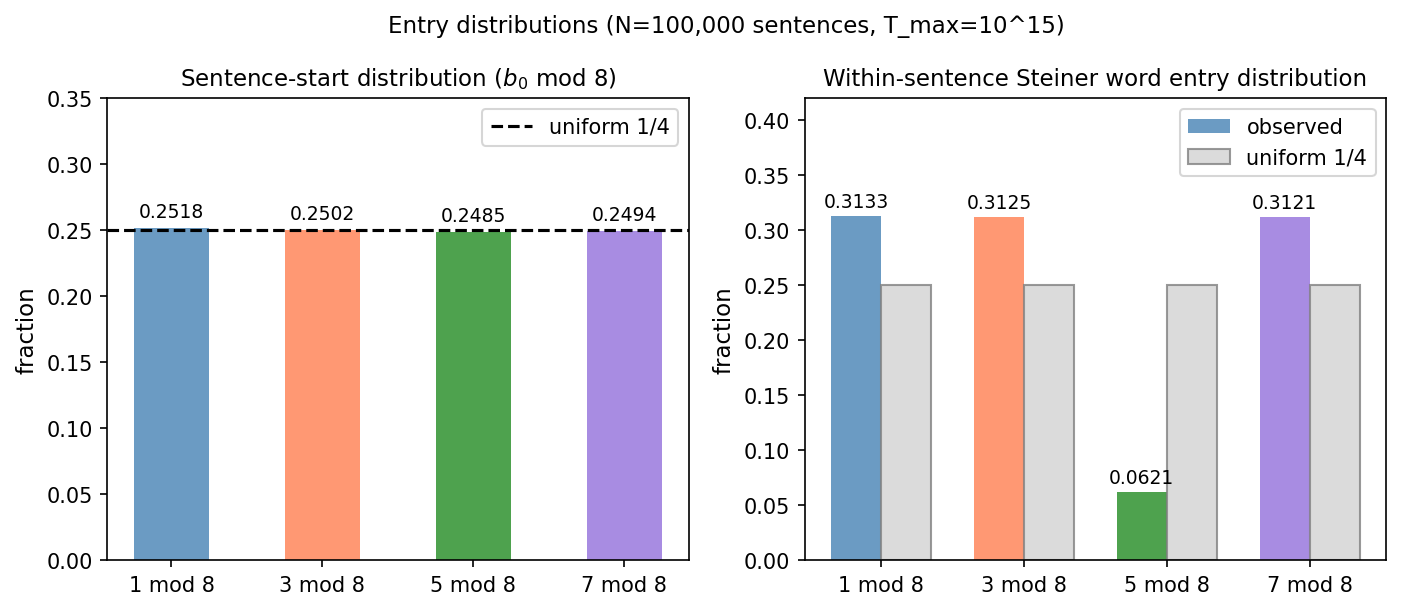
\includegraphics[width=\textwidth]{../65-branch-distribution/entry-distributions.png}
  \caption{Left: sentence-start distribution ($b_0 \bmod 8$) against the
  uniform $1/4$ baseline — confirmed uniform (Table~\ref{tab:start}).
  Right: within-sentence Steiner word entry distribution against the uniform
  $1/4$ baseline. Class~5 is structurally suppressed to ${\approx}6.2\%$
  (it can only appear as the terminal word); classes 1, 3, 7
  each carry ${\approx}31\%$.}
  \label{fig:entry}
\end{figure}

\subsection*{Sentence Length Distribution}

\begin{table}[h]
\centering
\begin{tabular}{rrrr}
\toprule
$k$ & Observed fraction & Naive $(1/2)^k$ & Theory $3^{k-1}/4^k$ \\
\midrule
 1 & 0.25180 & 0.50000 & 0.25000 \\
 2 & 0.18683 & 0.25000 & 0.18750 \\
 3 & 0.13931 & 0.12500 & 0.14063 \\
 4 & 0.10574 & 0.06250 & 0.10547 \\
 5 & 0.07844 & 0.03125 & 0.07910 \\
 6 & 0.05958 & 0.01563 & 0.05933 \\
 7 & 0.04490 & 0.00781 & 0.04449 \\
 8 & 0.03342 & 0.00391 & 0.03337 \\
 9 & 0.02490 & 0.00195 & 0.02503 \\
10 & 0.01866 & 0.00098 & 0.01877 \\
\bottomrule
\end{tabular}
\caption{Empirical Steiner sentence length distribution ($N=10^5$, $T_{\max}=10^{15}$)
vs.\ the naive $(1/2)^k$ prediction and the theoretical $3^{k-1}/4^k$
(Theorem~\ref{thm:main}). The naive prediction overestimates $P(k=1)$ by a
factor of~2 and decays far too fast for $k \geq 3$.}
\label{tab:lengths}
\end{table}

\begin{figure}[ht]
  \centering
  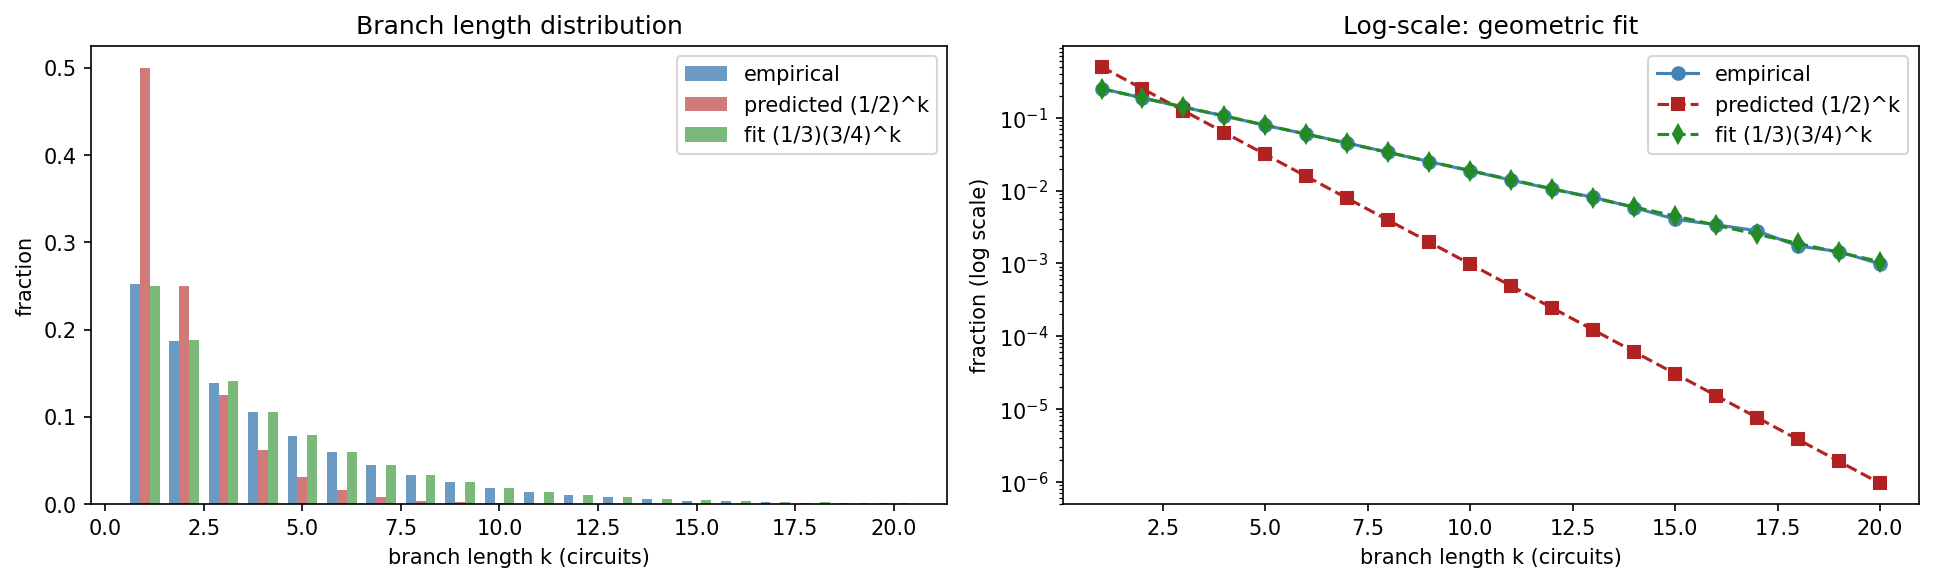
\includegraphics[width=\textwidth]{../65-branch-distribution/branch-length-distribution.png}
  \caption{Steiner sentence length distribution ($N=10^5$, $T_{\max}=10^{15}$):
  empirical (blue bars / circles) vs.\ naive $(1/2)^k$ (red) and theoretical
  $3^{k-1}/4^k$ (green), on linear scale (left) and log scale (right).
  On the log scale, the empirical slope matches $\log(3/4)$ precisely —
  not $\log(1/2)$. The naive prediction is dramatically refuted at $k=1$
  (predicts 50\%; observed 25\%) and for $k \geq 3$ (predicts too-fast decay).}
  \label{fig:lengths}
\end{figure}

\subsection*{Statistical Tests}

A $\chi^2$ goodness-of-fit test on 15 length bins plus a tail bin, using
$N = 10^5$ sentences:

\begin{center}
\begin{tabular}{lrrl}
\toprule
Model & $\chi^2$ & $p$-value & Verdict \\
\midrule
Naive $(1/2)^k$     & $1{,}022{,}029$ & $\approx 0$ & \textbf{Rejected} \\
Theory $3^{k-1}/4^k$ & $12.9$          & $0.61$      & Consistent \\
\bottomrule
\end{tabular}
\end{center}

The naive model is rejected with overwhelming confidence. The theoretical formula
$3^{k-1}/4^k$ is consistent with the data at all tested lengths.

% ---------------------------------------------------------------------------
\begin{thebibliography}{9}

\bibitem{paper33}
J.~Seymour,
\emph{A Regular Expression Language for the Collatz Graph} (Working Paper, Paper~33),
2026.

\bibitem{paper65}
J.~Seymour,
\emph{The $\frac{1}{3}(\frac{3}{4})^k$ Distribution of Steiner Sentence Lengths}
(Working Paper, Paper~65),
2026.

\bibitem{paper66}
J.~Seymour,
\emph{2-adic Valuations of $3n+1$ by Residue Class mod~8}
(Working Paper, Paper~66),
2026.

\end{thebibliography}

\end{document}
